\section{Exploring the segmentation by level sets}

In both examples (hand and brain) of the \texttt{levelset\_demo.m} the initial level set model is just a circumference that evolves depending on the gradient of the image and that finally adjusts to the desired anatomical shape: in the first case, the hand itself; in the second, the two small ventricular shapes in the center of the brain. In the second case the active contour is even able to modify its topology dividing into two contours. Although the source code for this example is already provided to us, we show, for the sake of illustration, the initial level set and the final contour for each of the two demonstrations in figure \ref{fig:levelset-demo}.

\begin{figure}[!hbt]
\centering   
\subfigure[Hand: levelset input]{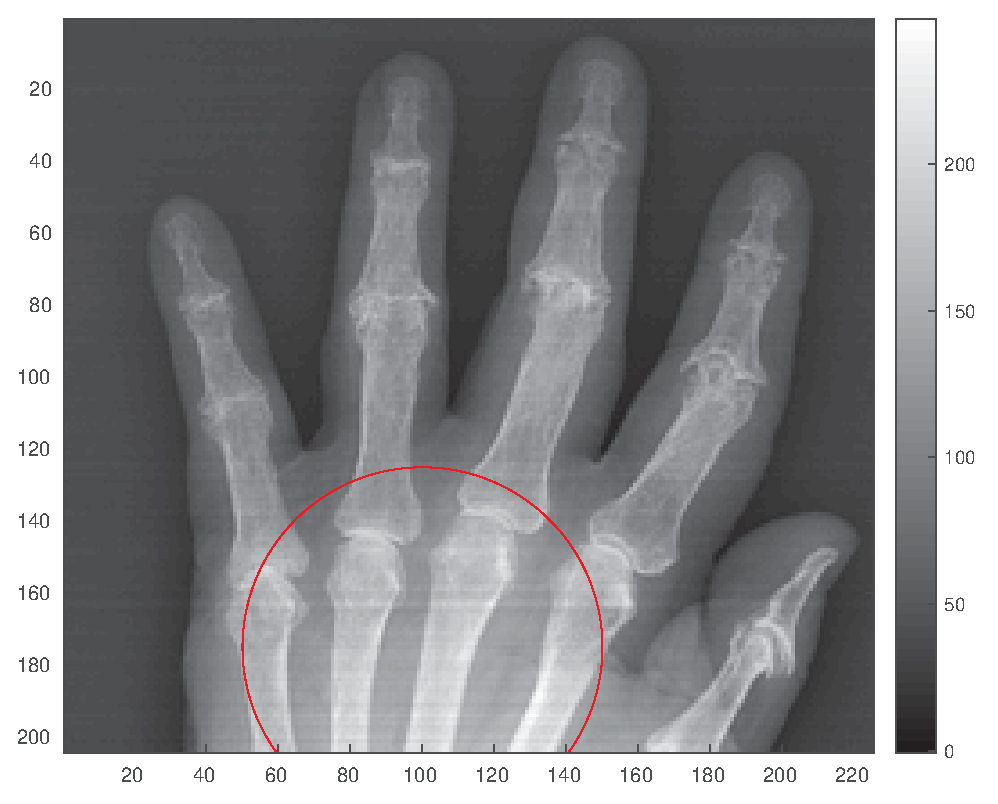
\includegraphics[width=60mm]{img/ex3/levelset_input.eps}}
\subfigure[Hand: levelset output]{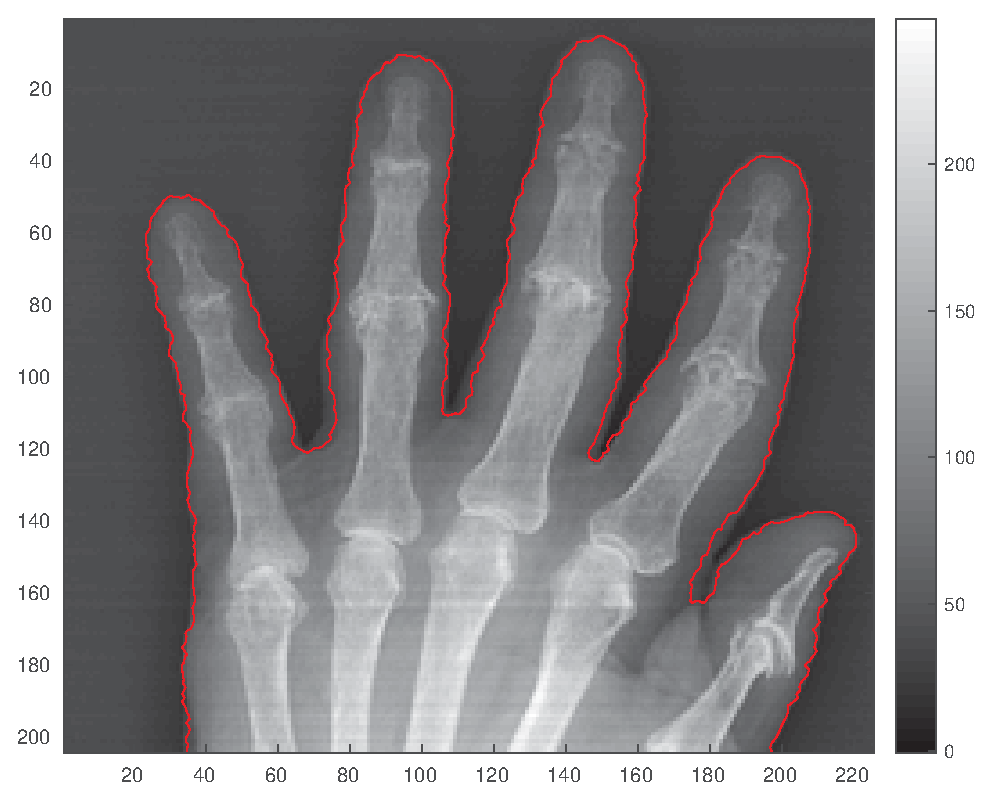
\includegraphics[width=60mm]{img/ex3/levelset_output.eps}}

\subfigure[Brain: levelset input]{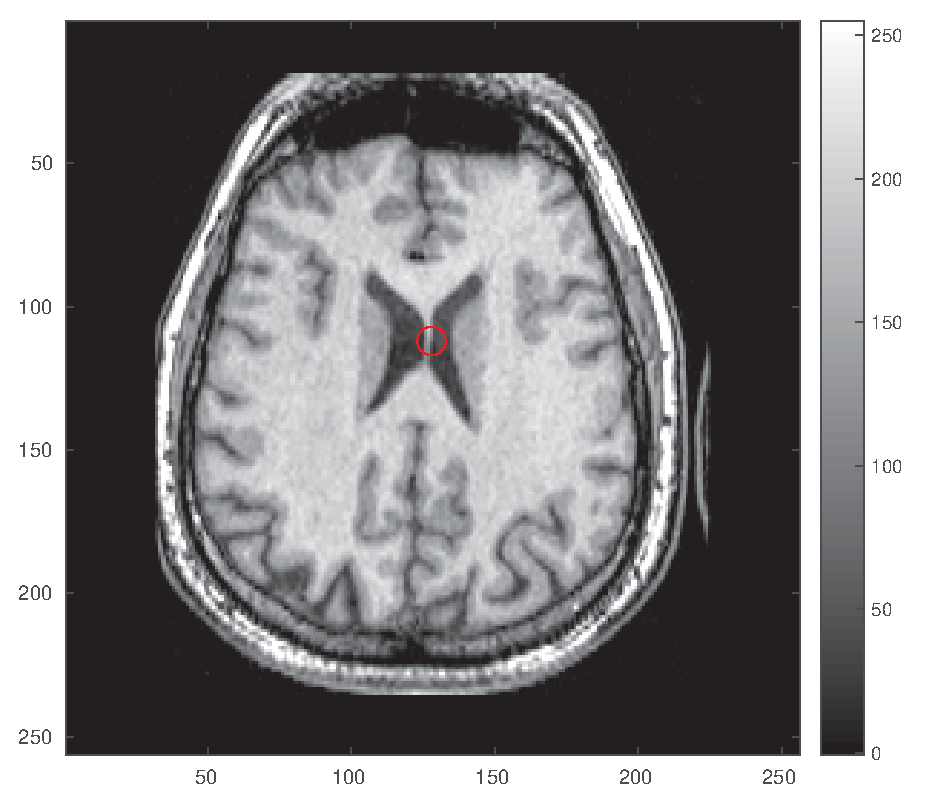
\includegraphics[width=60mm]{img/ex3/levelset_input2.eps}}
\subfigure[Brain: levelset output]{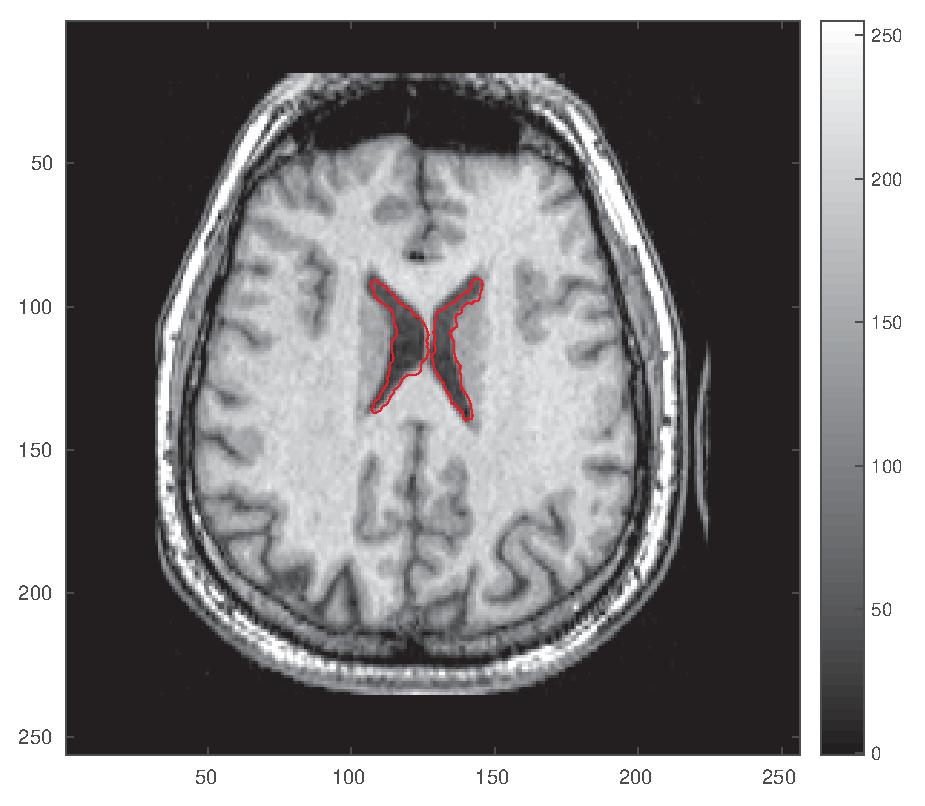
\includegraphics[width=60mm]{img/ex3/levelset_output2.eps}}

\caption{Initial and final contour for the first level set demo}
\label{fig:levelset-demo}
\end{figure}

The provided \texttt{levelset} method is an implementation of the level set segmentation algorithm by  Chan \& Vese\footnote{\textbf{T.F. Chan, L.A. Vese}\emph{An active contour model without edges}, Lecture Notes in Computer Science, vol. 1682, pp. 141-151, 1999}. This algorithm seeks to minimize the following energy functional:

\[ \min_{c_{in}, c_{out}, \Gamma} E(c_{in}, c_{out}, \Gamma \]
where $ E(c_{in}, c_{out}, \Gamma) = \mu \cdot \mathrm{Length}(\Gamma) + \nu \cdot \mathrm{Area}(\omega) + \lambda_{in} E_{in} (c_{in}, \Gamma) + \lambda_{out} E_{out} (c_{out}, \Gamma) $ is and energy functional (NOTE: $ \omega $ is the region inside the contour). In this expression, $ \mu $, $ \nu $, $ \lambda_{in} $ and $ \lambda_{out} $ are constant and govern the weight of the contour perimeter, the contour area and the internal and external energies in the overall functional. For instance, increasing $ \mu $ and reducing $ \nu $ can lead to contours with smaller perimeters and bigger areas or, in other words, closer to a circumference. On the other hand the internal and external energies model, respectively, how different is the outer gray level from the current $ c_{out} $ and the inner gray level from the current $ c_{in} $. Therefore $ \lambda_{in} $ and $ \lambda_{out} $ have to be tuned bearing this in mind. An initial contour and average intensities have to be given to the algorithm as well (the intensities can have an arbitrary value or can be initialized with the mean pixel intensity inside the contour boundary), so these appears as arguments of the \texttt{levelset} method as well. In the method the initial contour is inferred from the given \emph{level set function}, or $ \phi $, which measures the distance from each of the image pixels to the contour (positive outside the contour, negative inside).

Moreover the provided method takes the following additional parameters:
\begin{itemize}
	\item $ \kappa $: penalizes the difference between the current $ \phi $ and the distance function.
	\item $ \tau $: controls the displacement of the contour at each step. Can be increased for increased convergence speed or can be reduced if the iterations become erratic and or unstable.
	\item $ g $: modulates the weight of each pixel in the distance metric. By default is a full-one matrix.
\end{itemize}

The main difference between the segmentation of the brain in \texttt{levelset\_demo.m} and in \texttt{levelset\_demo2.m} is the initial location of the active contour. In the first example the contour is located in the center of the brain and therefore adjusts to the shape of the two ventricular shapes that are located in the middle. However in \texttt{levelset\_demo2.m} the contour is located outside and therefore it adjusts to the region with biggest area of the brain. Not surprisingly, the $ c_{in} $ and $ c_{out} $ are swapped accordingly while the rest are let as they are. We can see this in figure \ref{fig:levelset-demo}.

\begin{figure}[!hbt]
\centering   

\subfigure[Brain: levelset input]{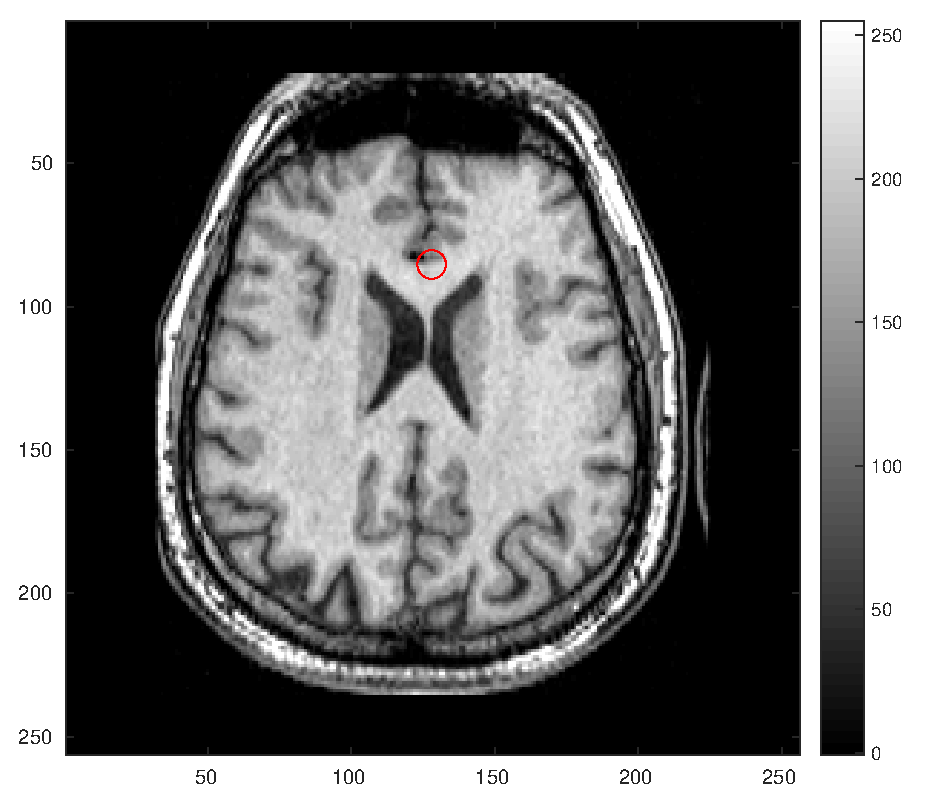
\includegraphics[width=60mm]{img/ex3/levelset_input2_outer.eps}}
\subfigure[Brain: levelset output]{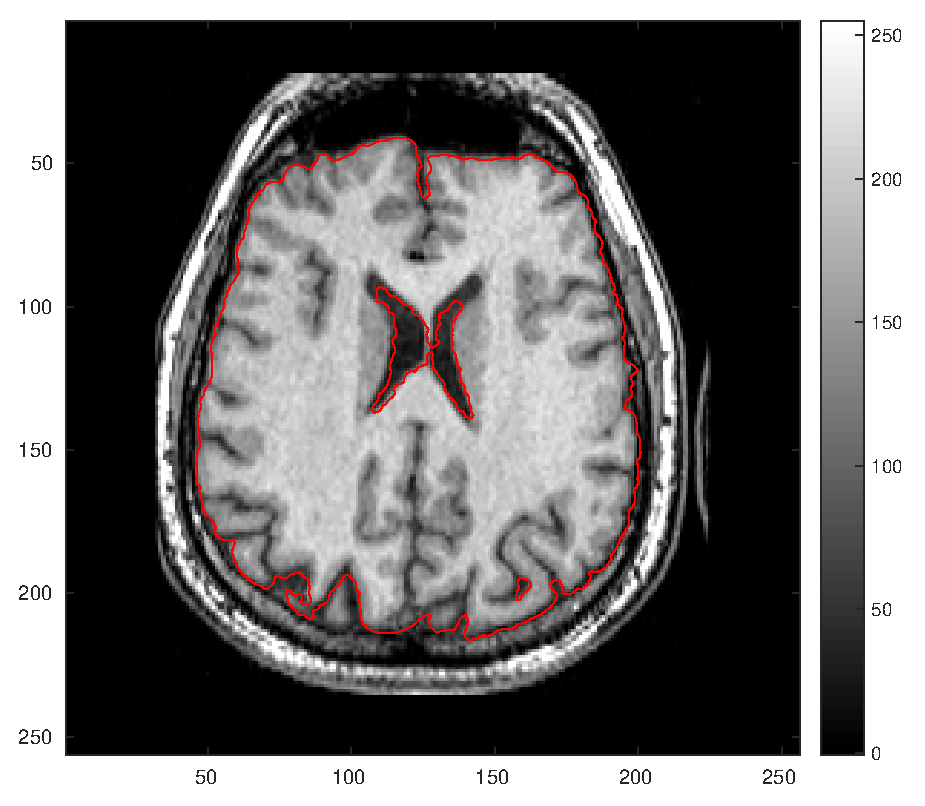
\includegraphics[width=60mm]{img/ex3/levelset_output2_outer.eps}}

\caption{Initial and final contour for the second level set demo}
\label{fig:levelset-demo2}
\end{figure}